
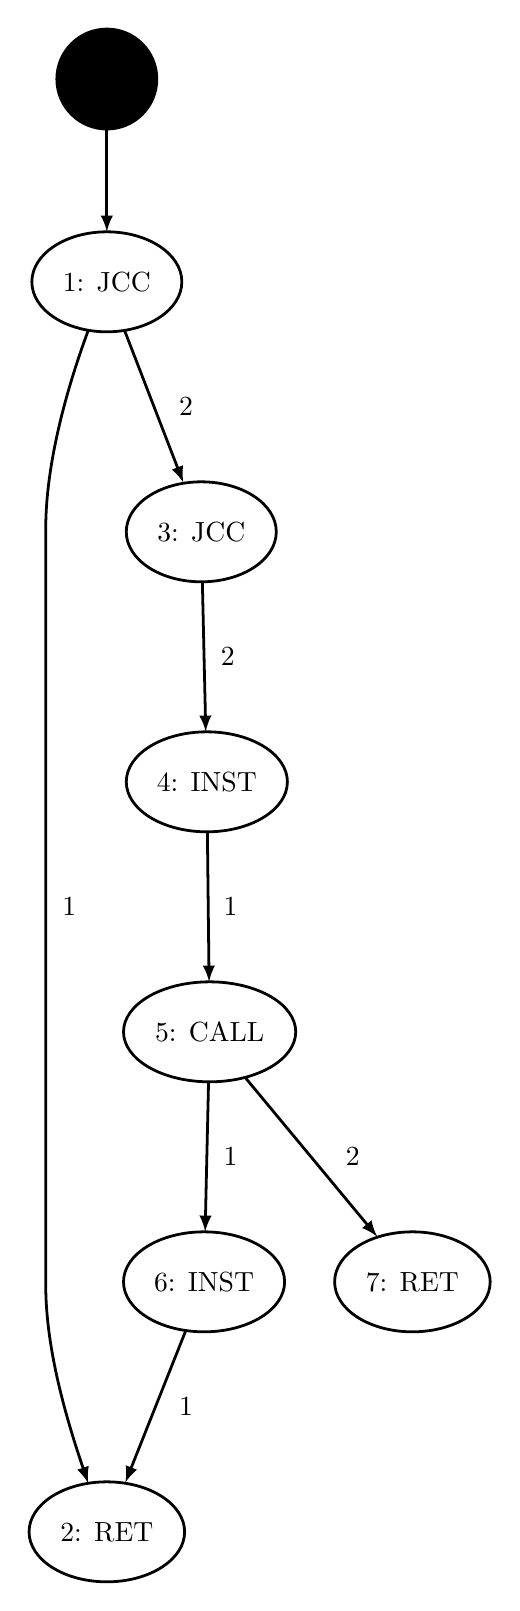
\begin{tikzpicture}[>=latex,line join=bevel,]
  \pgfsetlinewidth{1bp}
%%
\pgfsetcolor{black}
  % Edge: 2 -> 3
  \draw [->] (64.605bp,179.61bp) .. controls (64.324bp,167.24bp) and (63.94bp,150.37bp)  .. (63.388bp,126.05bp);
  \definecolor{strokecol}{rgb}{0.0,0.0,0.0};
  \pgfsetstrokecolor{strokecol}
  \draw (72.5bp,153.0bp) node {1};
  % Edge: 6 -> 7
  \draw [->] (62.395bp,359.61bp) .. controls (62.676bp,347.24bp) and (63.06bp,330.37bp)  .. (63.612bp,306.05bp);
  \draw (71.5bp,333.0bp) node {2};
  % Edge: 1 -> 6
  \draw [->] (34.395bp,450.45bp) .. controls (39.303bp,437.75bp) and (46.174bp,419.96bp)  .. (55.518bp,395.78bp);
  \draw (56.5bp,423.0bp) node {2};
  % Edge: 7 -> 2
  \draw [->] (64.198bp,269.61bp) .. controls (64.338bp,257.24bp) and (64.53bp,240.37bp)  .. (64.806bp,216.05bp);
  \draw (72.5bp,243.0bp) node {1};
  % Edge: 1 -> 4
  \draw [->] (21.28bp,450.44bp) .. controls (14.81bp,432.97bp) and (6.0bp,404.51bp)  .. (6.0bp,379.0bp) .. controls (6.0bp,379.0bp) and (6.0bp,379.0bp)  .. (6.0bp,107.0bp) .. controls (6.0bp,85.873bp) and (12.042bp,62.722bp)  .. (21.28bp,35.562bp);
  \draw (14.5bp,243.0bp) node {1};
  % Edge: 0 -> 1
  \draw [->] (28.0bp,522.81bp) .. controls (28.0bp,514.79bp) and (28.0bp,505.05bp)  .. (28.0bp,486.03bp);
  % Edge: 2 -> 5
  \draw [->] (78.051bp,181.27bp) .. controls (89.331bp,167.67bp) and (105.79bp,147.82bp)  .. (125.31bp,124.3bp);
  \draw (116.5bp,153.0bp) node {2};
  % Edge: 3 -> 4
  \draw [->] (56.417bp,90.448bp) .. controls (51.365bp,77.746bp) and (44.292bp,59.962bp)  .. (34.673bp,35.777bp);
  \draw (56.5bp,63.0bp) node {1};
  % Node: 1
\begin{scope}
  \definecolor{strokecol}{rgb}{0.0,0.0,0.0};
  \pgfsetstrokecolor{strokecol}
  \draw (28.0bp,468.0bp) ellipse (27.0bp and 18.0bp);
  \draw (28.0bp,468.0bp) node {1: JCC};
\end{scope}
  % Node: 0
\begin{scope}
  \definecolor{strokecol}{rgb}{0.0,0.0,0.0};
  \pgfsetstrokecolor{strokecol}
  \definecolor{fillcol}{rgb}{0.0,0.0,0.0};
  \pgfsetfillcolor{fillcol}
  \filldraw [opacity=1] (28.0bp,541.0bp) ellipse (18.0bp and 18.0bp);
\end{scope}
  % Node: 3
\begin{scope}
  \definecolor{strokecol}{rgb}{0.0,0.0,0.0};
  \pgfsetstrokecolor{strokecol}
  \draw (63.0bp,108.0bp) ellipse (29.0bp and 18.0bp);
  \draw (63.0bp,108.0bp) node {6: INST};
\end{scope}
  % Node: 2
\begin{scope}
  \definecolor{strokecol}{rgb}{0.0,0.0,0.0};
  \pgfsetstrokecolor{strokecol}
  \draw (65.0bp,198.0bp) ellipse (31.0bp and 18.0bp);
  \draw (65.0bp,198.0bp) node {5: CALL};
\end{scope}
  % Node: 5
\begin{scope}
  \definecolor{strokecol}{rgb}{0.0,0.0,0.0};
  \pgfsetstrokecolor{strokecol}
  \draw (138.0bp,108.0bp) ellipse (28.0bp and 18.0bp);
  \draw (138.0bp,108.0bp) node {7: RET};
\end{scope}
  % Node: 4
\begin{scope}
  \definecolor{strokecol}{rgb}{0.0,0.0,0.0};
  \pgfsetstrokecolor{strokecol}
  \draw (28.0bp,18.0bp) ellipse (28.0bp and 18.0bp);
  \draw (28.0bp,18.0bp) node {2: RET};
\end{scope}
  % Node: 7
\begin{scope}
  \definecolor{strokecol}{rgb}{0.0,0.0,0.0};
  \pgfsetstrokecolor{strokecol}
  \draw (64.0bp,288.0bp) ellipse (29.0bp and 18.0bp);
  \draw (64.0bp,288.0bp) node {4: INST};
\end{scope}
  % Node: 6
\begin{scope}
  \definecolor{strokecol}{rgb}{0.0,0.0,0.0};
  \pgfsetstrokecolor{strokecol}
  \draw (62.0bp,378.0bp) ellipse (27.0bp and 18.0bp);
  \draw (62.0bp,378.0bp) node {3: JCC};
\end{scope}
%
\end{tikzpicture}

